Последний рассмотренный метод -- SHAP. Ранее мы детально описали KernelSHAP, однако также упомянули TreeSHAP, который лучше подходит для моделей, в основе которых лежат решающие деревья. Оставим тот же самый объект, что мы рассматривали в LIME, и используем оба типа SHAP, чтобы сравнить качество и скорость.

\textbf{KernelSHAP}

\vspace{-1mm}
\begin{figure}[h]
	\centering{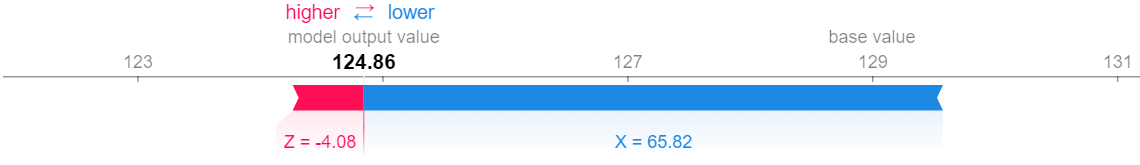
\includegraphics[width=\linewidth]{pics/shapxz.png}}
\end{figure}
\vspace{-5mm}

\textbf{TreeSHAP}

\vspace{-1mm}
\begin{figure}[h]
	\centering{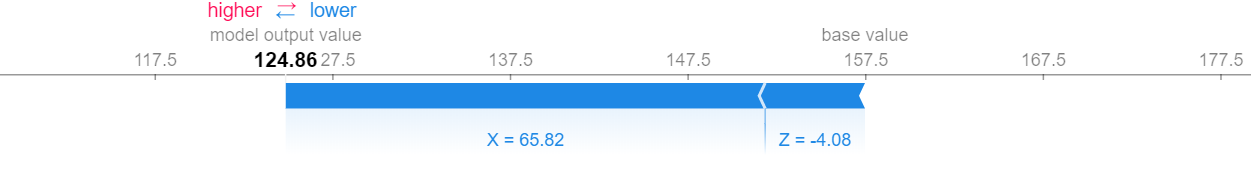
\includegraphics[width=\linewidth]{pics/shaptree.png}}
\end{figure}
\vspace{-5mm}

Мнения расходятся: KernelSHAP считает, что $Z$ положительно влияет на предсказание, TreeSHAP -- наоборот. Но оба сходятся на том, что $X$ оказывает большое отрицательное влияние, чем они отличаются от LIME. Однако стоит отметить, что LIME и SHAP по-разному рассчитывают некоторое исходное значение (base value), от которого отталкиваются при объяснении.

Тем не менее, результаты SHAP оказываются менее интуитивными. Значение $Z = -4.08$ должно увеличивать значение $y$, так как это лежит далеко от вершины параболы, причем за значением $25\%$ квартиля. Аналогично, $X$ -- чем больше $X$, тем сильнее наклон ветвей параболы --  в нашем случае $X$ лежит на границе $75\%$ квартиля, что уже почти выходит за пределы основной выборки. Все этом кажется говорит о том, что оба признака должны вносить положительный вклад в предсказание. Однако SHAP показывает совсем не такие результаты.

Для данной задачи рассматривалась небольшая выборка. Для нее KernelSHAP оказался быстрее TreeSHAP. Однако на большой выборке TreeSHAP выходит в лидеры (см. след. главу).

Далее рассмотрим только KernelSHAP, так как он предоставляет более точные результаты. Взглянем также на другие графики, которые предоставляет библиотека:

\begin{figure}[h]
	\centering{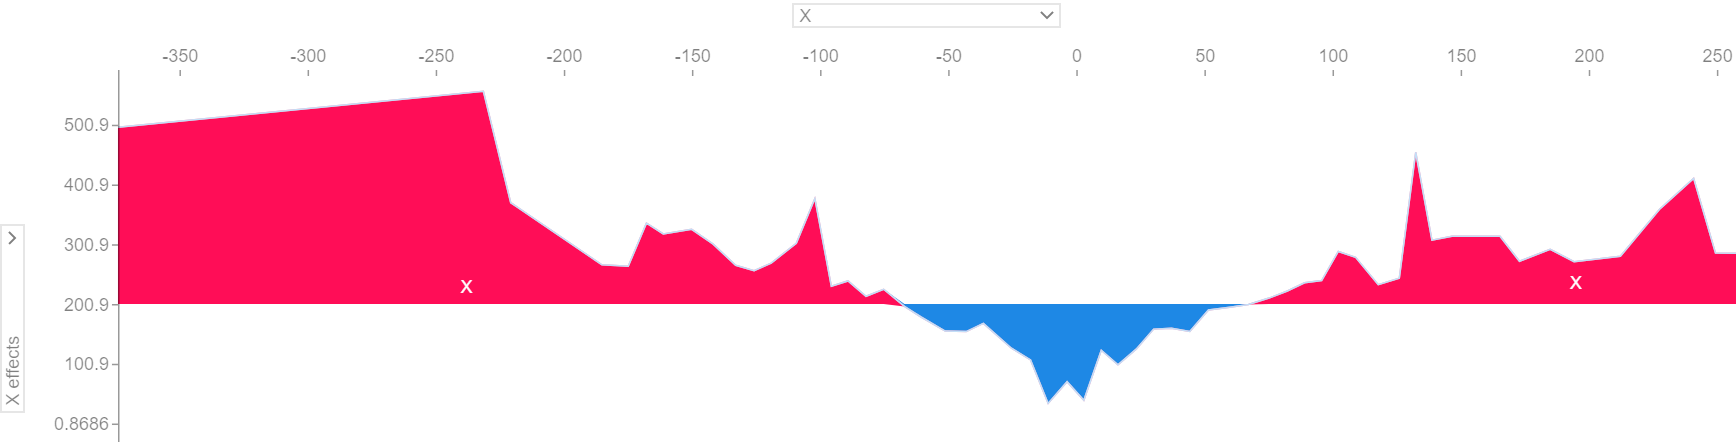
\includegraphics[width=0.90\linewidth]{pics/shapx.png}}
	\caption{Эффект признака X в зависимости от его значения}
\end{figure}
\vspace{-3mm}

\begin{figure}[h]
	\centering{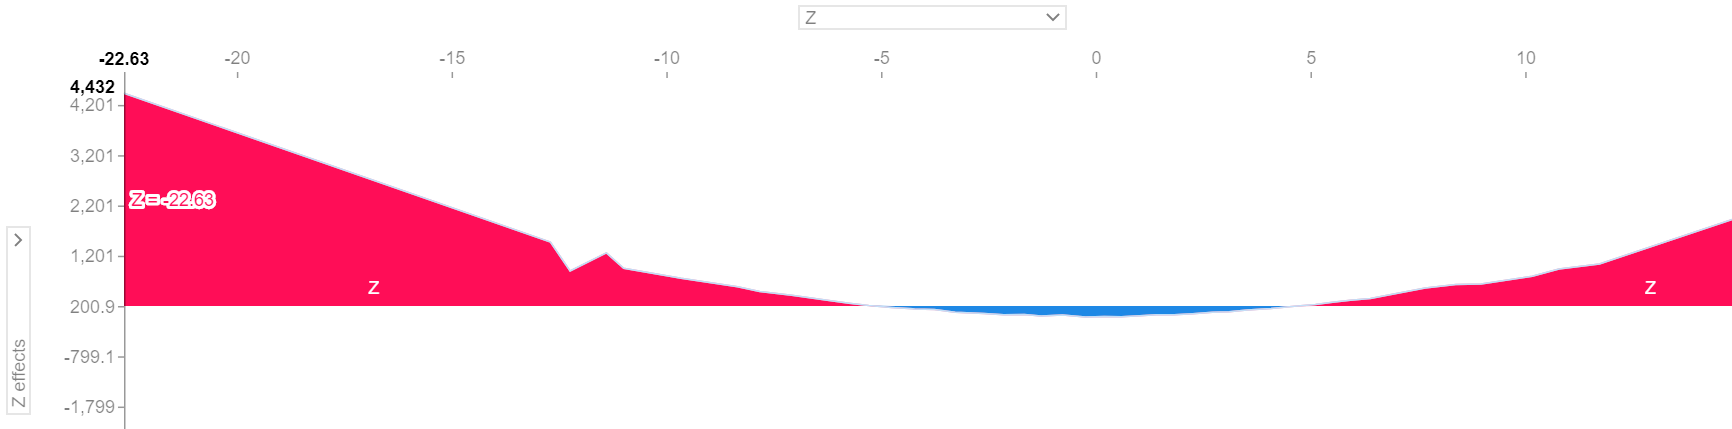
\includegraphics[width=0.9\linewidth]{pics/shapz.png}}
	\caption{Эффект признака Z в зависимости от его значения}
\end{figure}
\vspace{-3mm}

Оба графика являются аналогами PDP, которые мы строили ранее. Они отображают похожую картину, в случае признака $X$ даже более детализированную.

\begin{figure}[h]
	\centering{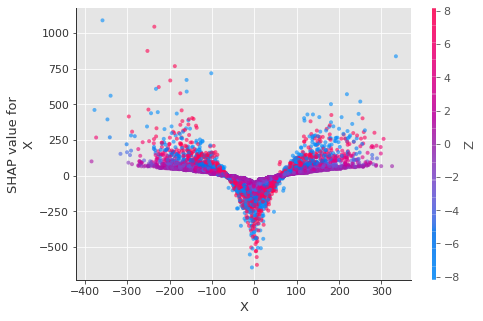
\includegraphics[width=0.6\linewidth]{pics/shapall.png}}
	\caption{Зависимость SHAP value признака X от его значения}
\end{figure}
\vspace{-3mm}

Еще одна альтернатива PDP от SHAP. Данный график показывает распределение признака $X$ и его SHAP value для разных объектов, а также его связь с признаком $Z$. По графику можно сделать следующий вывод: чем ближе значение $X$ к нулю, тем больше по модулю отрицательный вклад признака (его SHAP value); чем больше по модулю значение $X$, тем больше его положительный вклад. И есть две точки перегиба, в который вклад практически незаметен.

Цвет точек на графике показывает взаимосвязь с признаком $Z$ -- его шкала нарисована справа. Видно, что для низких и высоких значений $Z$ сохраняется одинаковая зависимость $y$ от $X$. Однако при $Z$, близком к нулю, значимость $X$ снижается и колеблется также около нуля. Данную зависимость действительно можно увидеть в исходных данных, но 3D-графику истинной функции $y$.

Получили, что SHAP не всегда дает точные результаты, к методу стоит относиться аккуратно. Тем не менее он предоставляет широкий функционал по анализу выборки, выполняет свои основные функции интерпретации и вылавливает зависимости, которые обнаружила модель в данных, хоть и с некоторой погрешностью.

Таким образом, все три метода решают поставленную задачу -- интерпретируют результат работы модели. Однако также все содержат определенную погрешность, из-за чего к объяснениям, полученным с помощью PDP, LIME и SHAP, стоит относиться осторожно, рассматривая разные точки зрения и обращая внимание на сами данные, смысл каждой переменной.